\clearpage
\subsection{Parte 2: Circuito RL in corrente impulsata - inversione del segno della tensione del generatore tra $-V_0$ e $+V_0$}

\subsubsection{Cenni Teorici}
%
Per la seconda legge di Kirchhoff, l'equazione del circuito RL è:
$$ V_{Resistore} + V_{Induttore} = V_{generatore} $$
Si ha che $ V_{Resistore} = V_R = RI$ e $ V_{Induttore} = V_L = L \frac{\mathrm d I }{\mathrm d t} $, dunque:
$$ RI + L \frac{\mathrm d I }{\mathrm d t} = V_{generatore} $$
%
\subsubsection*{Passaggio da $-V_0$ a $+V_0$}
Si ha $V_{generatore} = V_0$, e la condizione iniziale $I(t=0) = -\frac{V_0}{R} $ (poiché un istante prima il generatore eroga $-V_0$).\\
Usando il metodo della separazione delle variabili, e ponendo $\tau = \frac{L}{R} $, si trova la soluzione:
$$ I(t) = \frac{V_0}{R}(1-2e^{-\frac{t}{\tau}})$$
Da cui:
\[
  \begin{cases}
    V_R(t) = I(t) R = V_0(1-2e^{-\frac{t}{\tau}})\\
    V_L(t) = V_0 - V_R(t) = 2 V_0 e^{-\frac{t}{\tau}}\\
  \end{cases}
\]


\subsubsection*{Passaggio da $+V_0$ a $-V_0$}
Si ha $V_{generatore} = -V_0$, e la condizione iniziale $I(t=0) = \frac{V_0}{R} $ (poiché un istante prima il generatore eroga $+V_0$).\\
Come prima, usando il metodo della separazione delle variabili, e ponendo $\tau = \frac{L}{R} $, si trova la soluzione:
$$ I(t) = -\frac{V_0}{R}(1-2e^{-\frac{t}{\tau}})$$
Da cui:
\[
  \begin{cases}
    V_R(t) = I(t) R = -V_0(1-2e^{-\frac{t}{\tau}})\\
    V_L(t) = V_0 - V_R(t) = -2 V_0 e^{-\frac{t}{\tau}}\\
  \end{cases}
\]

\newpage
\subsubsection{Analisi dati}
Seguono qui i dati fittati con le equazioni appena ricavate.\\
%
% Grafico RL
%
    \begin{figure}[H]
    \centering
    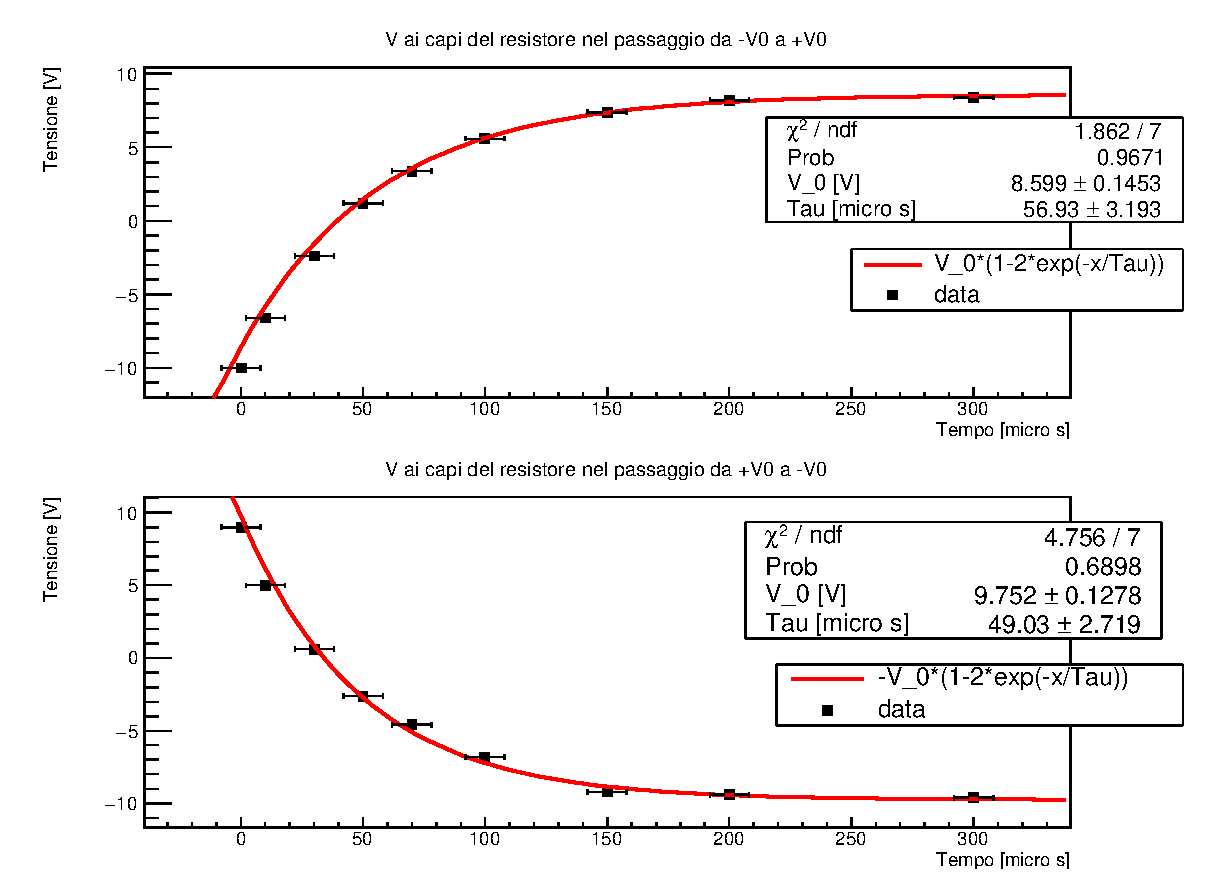
\includegraphics[scale=0.8]{Grafici/C3_P2_RL_impulsata_resistore.eps}
    %\caption{}
    \end{figure} 
%
    \begin{figure}[H]
    \centering
    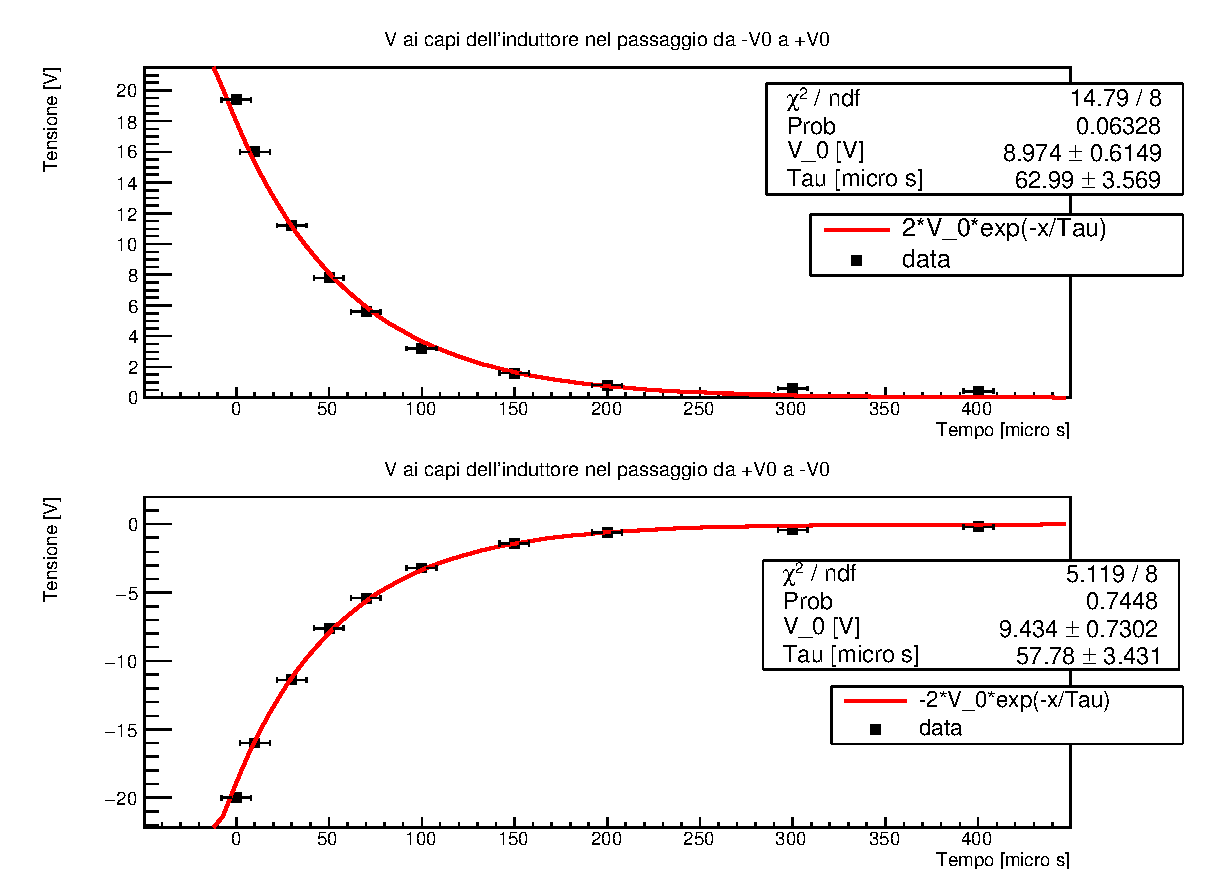
\includegraphics[scale=0.8]{Grafici/C3_P2_RL_impulsata_induttore.eps}
    %\caption{}
    \end{figure} 
%
%
La resistenza usata è $677 \pm 7$ Ohm (l'errore è stato calcolato come indicato sul manuale tecnico dello strumento).\\\\
%
%
Si ottiene il valore di $\tau$ con il suo errore calcolando la media pesata dei quattro valori ottenuti dai quattro fit (vedi fine paragrafo)
%
Si ricava il valore dell'induttanza $L$ e il suo errore, conoscendo la relazione $\tau = \frac{L}{R}$ e utilizzando la formula di propagazione dell'errore.\\

Risultati ottenuti:
$$\tau = 56 \pm 2 \mu s $$
$$ L = 0.038 \pm 0.001  H$$
